\documentclass[a4paper,12pt]{article}
\usepackage[margin=0.75in]{geometry}
\usepackage[utf8]{inputenc}
\usepackage[backend=bibtex]{biblatex}
\usepackage{graphicx}
\usepackage{titling}
\usepackage{titlesec}
\usepackage{placeins}
\addbibresource{references.bib}

\newcommand{\imagesource}[1]{{\footnotesize Sumber: #1}}
\renewcommand{\contentsname}{Daftar Isi}
\renewcommand{\thefigure}{\arabic{section}.\arabic{figure}}
\renewcommand{\figurename}{Gambar}

\titleformat{\section}
  {\normalfont\Large\bfseries}{Bab. \thesection}{1em}{}

\begin{document}
\begin{titlepage}
\begin{center}
\textbf{\huge Proposal Penelitian}\vspace{1cm}

\textbf{\Large Tentang}\vspace{1cm}

\textbf{\LARGE Purwarupa Implementasi Kubernetes Menggunakan Raspberry Pi untuk Menciptakan Lingkungan Peluncuran Aplikasi Web yang Dapat Diskala}\vspace{3cm}


\includegraphics[width=2in]{pictures/cover_ub.png}\vspace{3cm}

\textbf{\large Oleh:}\vspace{0.5cm}

Gabrielle Evan Farrel\vspace{0.25cm}

Reza Andria Siregar, S.T., M.Kom\vspace{1cm}

\textbf{\Large Fakultas Ilmu Komputer}

\textbf{\Large Universitas Brawijaya}

\textbf{\Large Malang 2023}
\end{center}
\end{titlepage}

\begin{center}
{\Large \textbf{HALAMAN PENGESAHAN}}
\end{center}

\begin{enumerate}
\item[a.] Judul Penelitian : Purwarupa Implementasi Kubernetes Menggunakan Raspberry\\
\phantom{Judul Penelitian :} Pi untuk Menciptakan Lingkungan Peluncuran Aplikasi Web\\
\phantom{Judul Penelitian :} yang Dapat Diskala
\item[b.] Bidang Ilmu : Komputasi Berbasis Jaringan
\item[c.] Peneliti Utama
\begin{itemize}
\item Nama : Gabrielle Evan Farrel
\item NIM : 205150201111033
\end{itemize}
\item[d.] Anggota Peneliti
\begin{itemize}
\item Nama : Reza Andria Siregar, S.T., M.Kom
\item NIP/NIDN : 197906212006041003/0021067909
\item Bidang Keahlian : Jaringan Nirkabel
\end{itemize}
\item[e.] Mahasiswa Peneliti
\begin{itemize}
\item Nama : Muhammad Muhajir Kurniawan
\item NIM : 165150207111043
\item Nama : Haidar Harfi Hadhiansah
\item NIM : 205150209111005
\end{itemize}
\item[f.] Waktu Penelitian : 6 bulan (Mei – Oktober 2022)
\item[g.] Biaya Penelitian
\begin{itemize}
\item Sumber DIPA : Rp 9.900.000, -
\item Sumber Lain : -
\item Total : Rp 9.900.000, -
\item Terbilang : Sembilan juta Sembilan ratus ribu rupiah
\end{itemize}
\end{enumerate}

\begin{flushright}
Malang, 4 Februari 2023 \hspace{2.5cm}

Peneliti \hspace{5.4cm}
\vspace{1.5cm}

Gabrielle Evan Farrel \hspace{3.04cm}

NIM. 205150201111033 \hspace{2.74cm}

\end{flushright}

\begin{flushleft}
Mengetahui \hspace{7.7cm} Menyetujui \\
Dekan FILKOM \hspace{6.85cm} Ketua BPPM FILKOM \\
\vspace{1.5cm}
Wayan Firdaus Mahmudy, S.Si., M.T., Ph.D \hspace{1.7cm} Bayu Rahayudi, M.T., M.M \
NIP. 197209191997021001 \hspace{6.05cm} NIP. 197407122006041001    
\end{flushleft}

\section*{Abstrak}
Implementasi Kubernetes pada Raspberry Pi untuk menciptakan lingkungan peluncuran aplikasi web yang dapat didiskalakan akan diteliti dan diuji coba. Dengan tujuan membuktikan bahwa Kubernetes dapat dioperasikan pada perangkat keras yang lebih kecil seperti Raspberry Pi dan menciptakan lingkungan peluncuran aplikasi web yang efisien dan dapat didiskalakan. Hasil dari penelitian ini akan dipresentasikan dalam bentuk dokumentasi yang memudahkan pemahaman dan mengimplementasikan kluster Kubernetes sendiri menggunakan Raspberry Pi dan Ansible untuk otomatisasi. Dengan demikian, proyek ini bertujuan untuk memperkaya pengetahuan dan memberikan solusi praktis bagi mereka yang ingin belajar membuat kluster Kubernetes dengan Ansible dan menggunakan K3s sebagai server.
\addcontentsline{toc}{section}{Abstrak}

\begin{flushleft}
KATA KUNCI : Kubernetes, Raspberry Pi, K3s, Ansible, otomatisasi, kluster 
\end{flushleft}
\newpage

\tableofcontents
\newpage

% \section{Pendahuluan}
\subsection{Latar Belakang}
Klustering seiring berjalannya waktu semakin banyak digunakan di kalangan perusahaan tekno-logi. hal tersebut terjadi karena kemudahan yang diberikan oleh teknologi ini, untuk melakukan skalasi layanan dengan terhadap peluncuran perangkat lunak kepada konsumen setiap kali kebutuhan bertambah. Dimana dengan berkembangnya zaman digital, kebutuhan manusia untuk mendapatkan semakin banyak kekuatan komputasi semakin tidak dapat dielakkan. Tetapi terdapat batasan skalasi secara vertikal (menambah RAM, menambah CPU, menambah penyimpanan persisten di dalam satu sistem).

\vspace{0.2cm}
\noindent Dengan harga komoditas yang dibutuhkan sebagai bahan dasar pembuatan produk elektronik, inflasi, dan peningkatan biaya produksi barang elektronik, maka skalasi secara vertikal akan menjadi semakin sulit seiring dengan peningkatan harga komponen yang disebabkan oleh kualitas yang dibutuhkan \cite{electronic_cost}. Hal ini menyebabkan bertambahnya penggunaan perangkat komputasi murah yang dapat dengan mudah di produksi masal. dan diprediksi akan semakin meningkat seiring dengan berjalannya waktu \cite{raspi_market}.

\vspace{0.2cm}
\noindent Dengan meningkatnya penggunaan klustering, diperlukan pula sebuah sistem yang mampu memberikan solusi untuk pengelolaan node pada sebuah kluster yang dapat di otomatisasi. sehingga dapat dilakukan peluncuran aplikasi kepada konsumen secara efektif. Dan sistem tersebut harus mampu mengatasi \textit{error} ketika melakukan tugas yang telah diberikan sebelumnya, sehingga kemungkinan kerusakan terhadap seluruh jajaran sistem dapat dihindari.


\subsection{Rumusan Masalah}

\subsection{Tujuan}

\subsection{Manfaat}

\subsection{Batasan Masalah}
% \section{Tinjauan Pustaka}

Kluster Merupakan sebuah teknologi yang dibuat sebagai upaya untuk mendapatkan kemampuan komputasi besar dengan harga murah. hal ini dilakukan dengan cara menghubungkan komputer, baik \textit{standalone}, terdistribusi, maupun paralel, dengan tujuan untuk membagi pekerjaan yang sebelumnya hanya dapat dilakukan oleh satu komputer saja secara bersamaan \cite{cloud_computing}. Untuk membagi tugas didalam setiap node, digunakan teknologi yang bernama Kontainerisasi.

\vspace{0.2cm}
\noindent Kontainerisasi memberikan kemampuan kepada pengembang untuk menciptakan aplikasi port-able \cite{containers}. menggunakan kontainerisasi, sebuah node dapat menjalankan berbagai macam tugas secara bersamaan, tanpa perlu mengkhawatirkan terjadinya konflik antar proses mengenai sumber daya yang ada. Seperti versi program yang berbeda, pustaka program yang tidak dapat ada secara bersamaan, dan kebutuhan akan integrasi kuat antar program di dalam kontainer. Selain itu, terdapat pula faktor keamanan dimana ketika sebuah kontainer terkontaminasi atau terkena serangan eksternal, tidak akan terjadi kerusakan pada kontainer lain karena isolasi yang diberikan oleh teknologi ini.

\vspace{0.2cm}
\noindent Penggunaan Raspberry Pi dalam server sederhana dan perangkat keras komputer juga meningkat seiring dengan berjalannya waktu. hal ini disebabkan oleh semakin tingginya angka pengembang aplikasi yang membutuhkan perangkat IoT dan lingkungan pengembangan murah untuk didapatkan dan/atau untuk digunakan sebagai sarana pembelajaran \cite{raspi_market}.

\subsection{Kubernetes}

Kubernetes memberikan sebuah platform open source portabel yang dapat diperluas untuk mengelola beban kerja dan layanan dalam container dalam bentuk orkestrasi, yang memfasilitasi konfigurasi deklaratif dan otomatisasi \cite{kubernetes_overview}. Didalamnya, terdapat Kluster, yang terdiri dari sekumpulan mesin pekerja, yang disebut node, yang menjalankan aplikasi dalam container. Setiap cluster memiliki setidaknya satu node pekerja \cite{kubernetes_components}. Node sendiri adalah sebuah perangkat keras maupun virtual yang bertugas menjalankan program didalam kontainer yang disebut Pods yang diluncurkan kedalam kluster yang diatur oleh sebuah \textit{controlplane} \cite{kubernetes_nodes}. Komponen komponen tersebut bersinergi dan bekerja sama dalam membentuk lingkungan perangkat lunak yang dapat terskala dan tumbuh secara horizontal. Sehingga dapat memberikan peluang baru bagi pengembang aplikasi dan administrator untuk merubah daya komputasi sesuai kebutuhan aplikasi pada saat tertentu dengan mudah dan mempermudah implementasi \textit{redundancy}.\\
\begin{figure}[htb!]
    \centering
    \begin{tabular}{ @{} r @{} }
        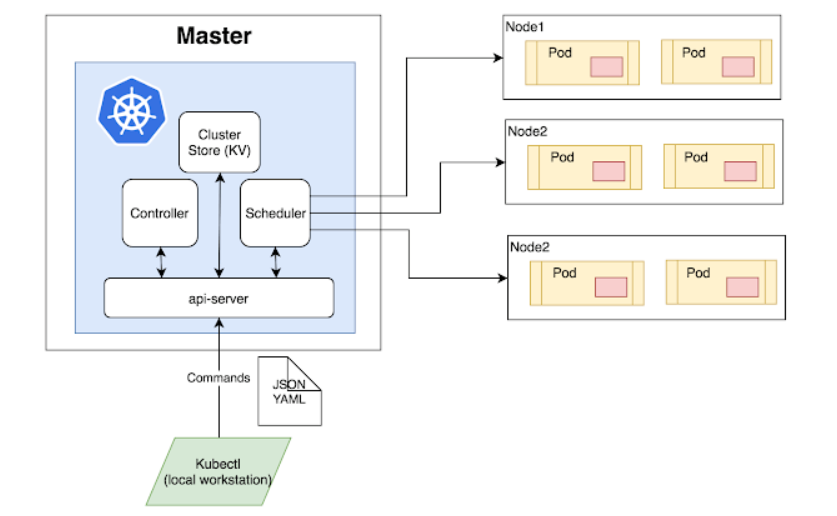
\includegraphics[scale=0.7]{pictures/k8s_diagram.png}\\
        \imagesource{https://www.eternalsoftsolutions.com}
    \end{tabular}
    \caption{Struktur Kubernetes (K8s)}
\end{figure}
\FloatBarrier

\subsection{Raspberry Pi}

Raspberry Pi adalah komputer kecil menggunakan arsitektur ARM murah yang berfungsi seperti komputer pada umumnya \cite{raspi}. Perangkat keras ini memberikan akses komputasi murah untuk menciptakan perangkat-perangkat lain seperti Internet of Things (IoT), Personal Computer (PC), dan Server. Dan karena mudahnya mendapatkan perangkat dalam jumlah yang besar, maka Raspberry Pi juga dapat digunakan sebagai node untuk dihubungkan menggunakan Kubernetes dengan K3s.
\begin{figure}[htb!]
    \centering
    \begin{tabular}{ @{} r @{} }
        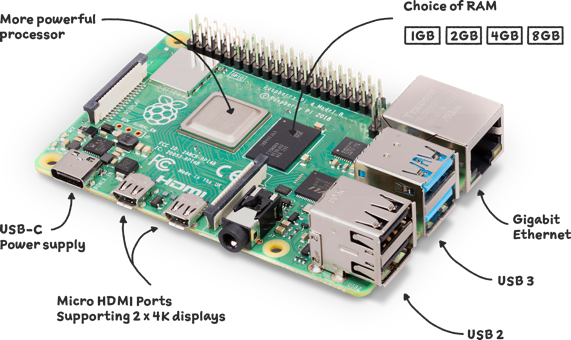
\includegraphics[scale=0.4]{pictures/raspi.png}\\
        \imagesource{https://www.raspberrypi.com/}
    \end{tabular}
    \caption{Komponen Raspberry Pi 4B}
\end{figure}
\FloatBarrier

\subsection{K3s}

K3s merupakan salah satu distribusi Kubernetes tersertifikasi dengan ketersediaan tinggi yang dirancang untuk beban kerja produksi di lokasi terpencil yang tidak diawasi, terbatas sumber daya, atau di dalam peralatan IoT \cite{k3s}. Portabilitas, ketersediaan, dan keringanan yang dimiliki oleh K3s didapatkan dengan memanfaatkan enkapsulasi seluruh komponen nya dalam satu proses. Yang hanya membutuhkan setidaknya 1vCPU dan 512MB RAM \cite{k3s_mk8s}. minimnya penggunaan sumber daya juga menjadi alasan utama pemilihan K3s jika dibandingkan dengan teknologi serupa seperti mK8s (MicroK8s) \cite{k3s_mk8s}. Dan karena enkapsulasi itu pula, tidak dibutuhkan pemasangan \textit{Docker Engine} secara terpisah didalam sistem yang menjalankan K3s.\\
\begin{figure}[htb!]
    \centering
    \begin{tabular}{ @{} r @{} }
        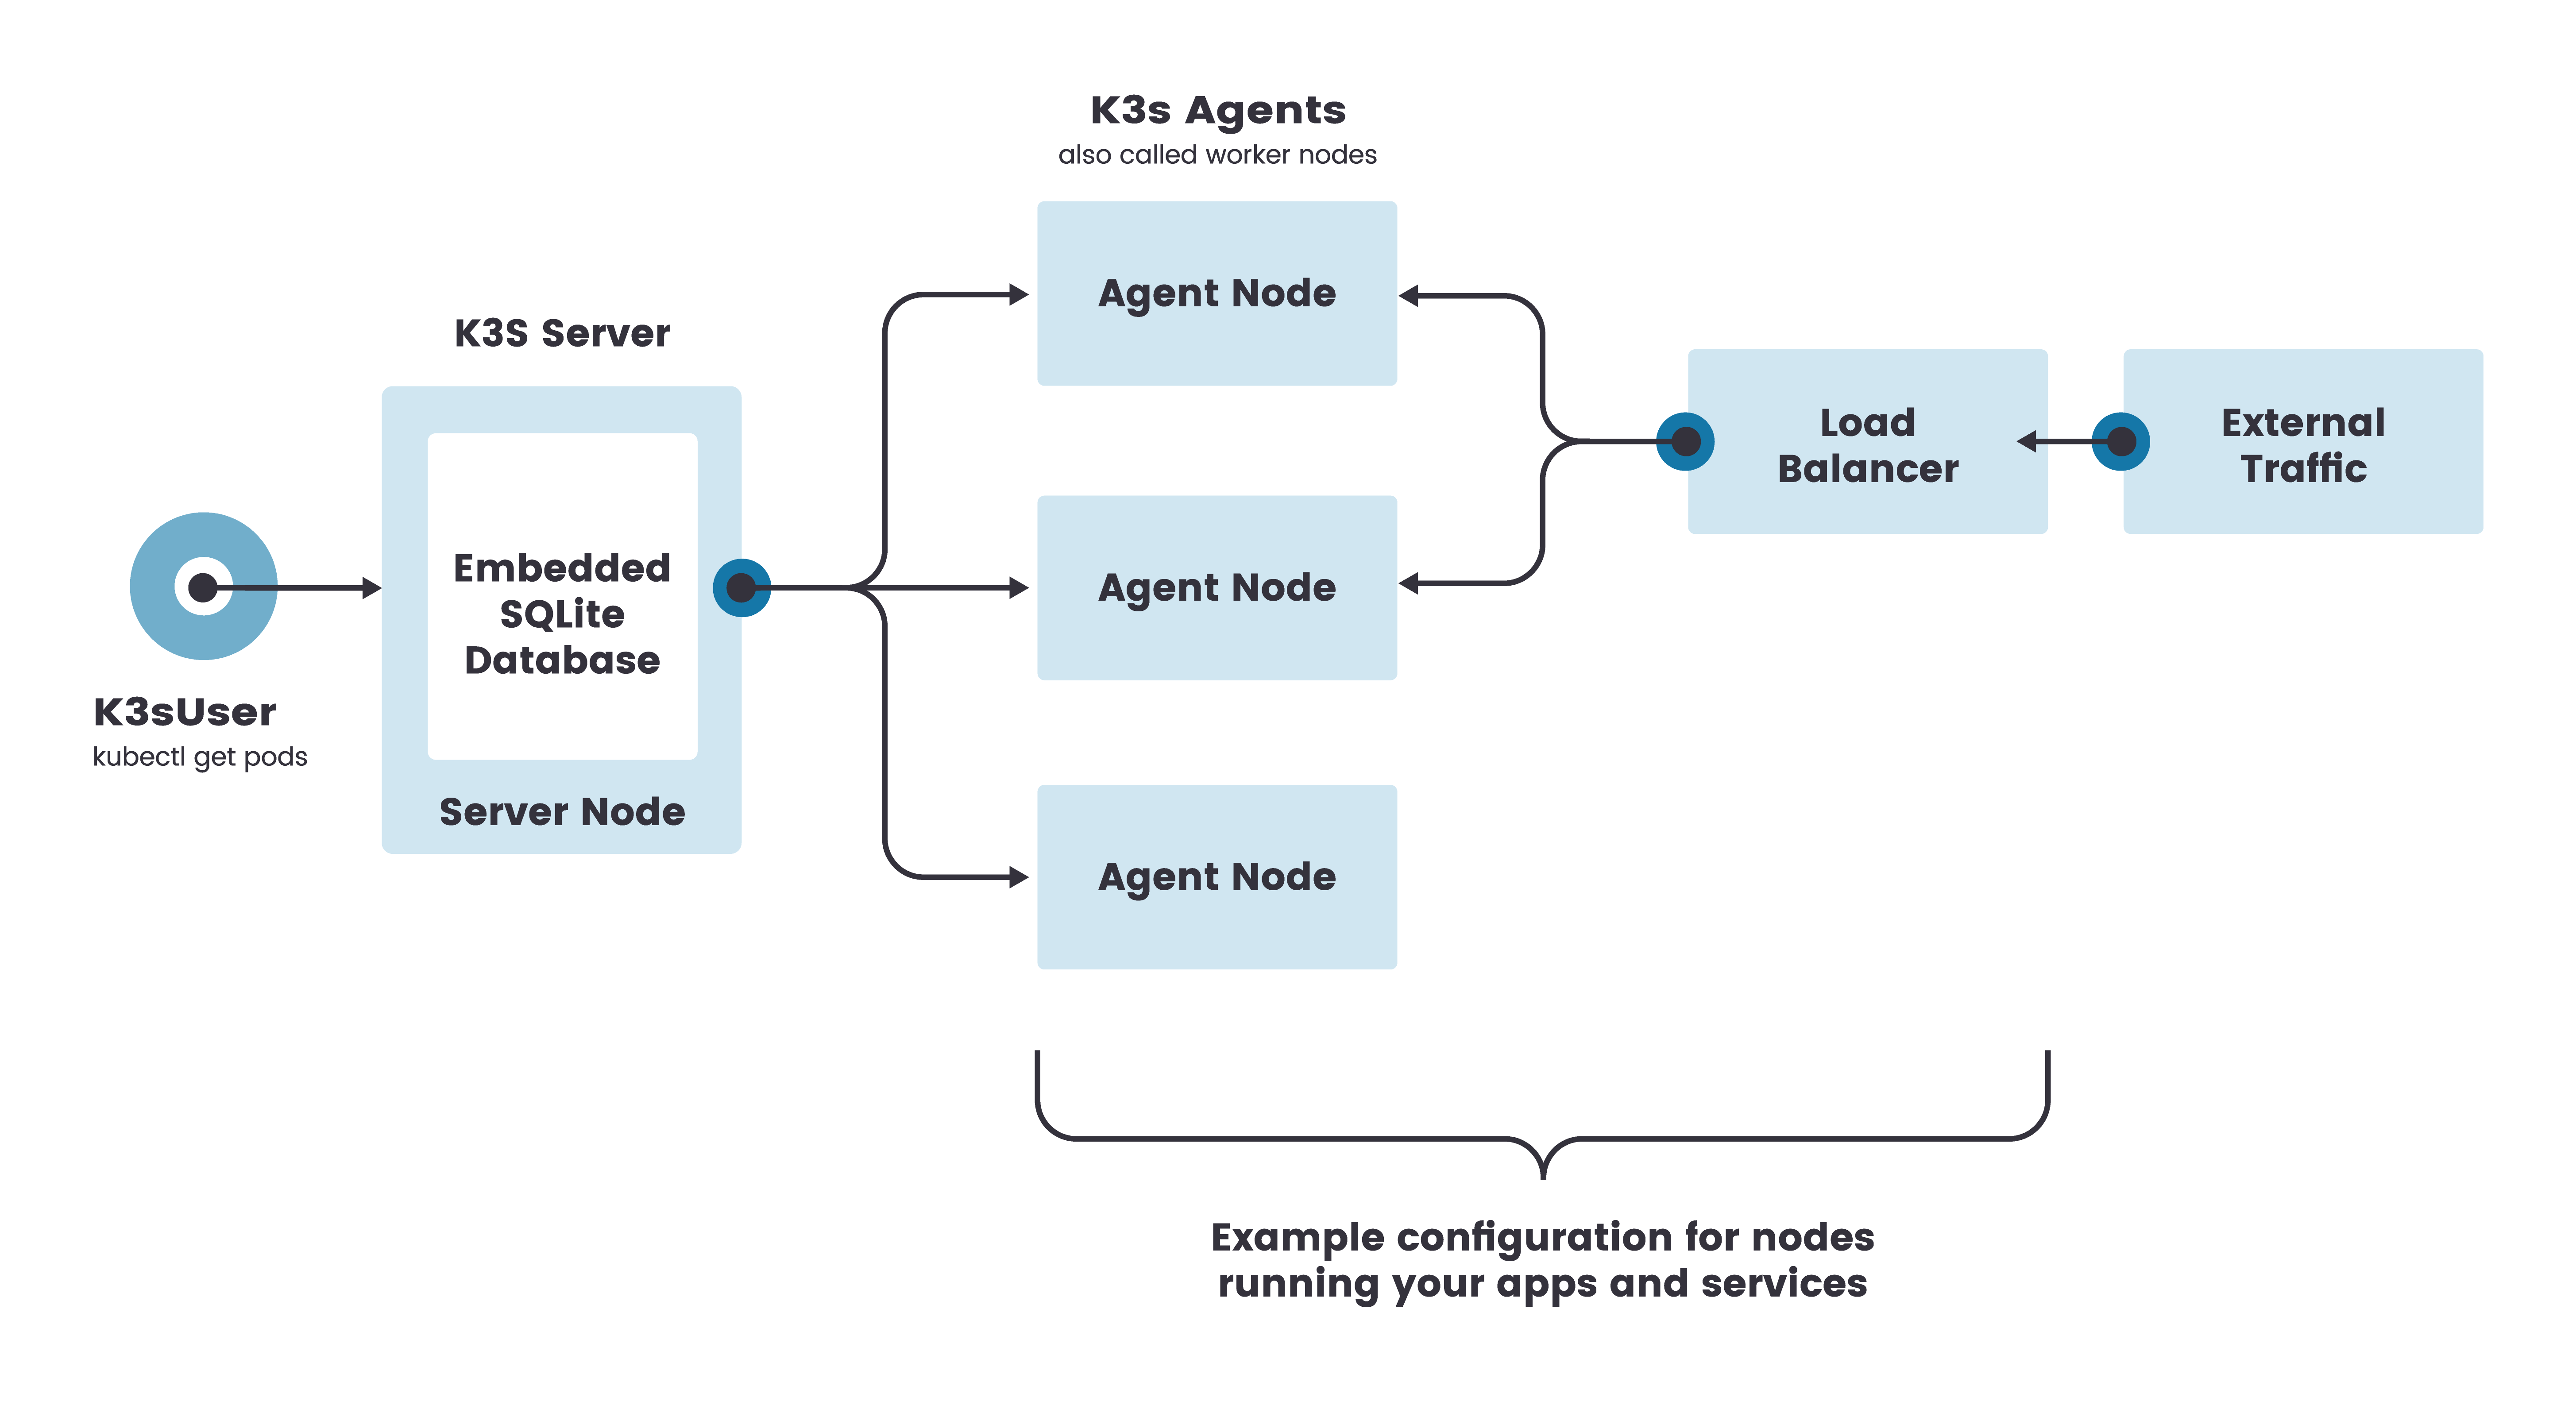
\includegraphics[scale=0.28]{pictures/k3s_diagram.png}\\
        \imagesource{https://nimblehq.co}
    \end{tabular}
    \caption{Struktur K3s}
\end{figure}
\FloatBarrier

\subsection{Ansible}

Ansible memiliki kemampuan untuk menghubungkan dan mempermudah proses pengaturan dan perawatan sistem pada saat peluncuran aplikasi. Karena Ansible mampu melakukan konfigurasi sistem, peluncuran perangkat lunak, dan mampu melakukan orkes-trasi kegiatan teknologi seperti \textit{Circular Integration/Circular Deployment} (CI/CD) \cite{ansible_docs}. menggunakan Ansible, pengaturan berulang yang harus dilakukan untuk setiap Node Rapsberry-Pi dapat di otomatisasi sehingga dapat mengurangi \textit{human error} dan meningkatkan efektifitas waktu.\\
\begin{figure}[htb!]
    \centering
    \begin{tabular}{ @{} r @{} }
        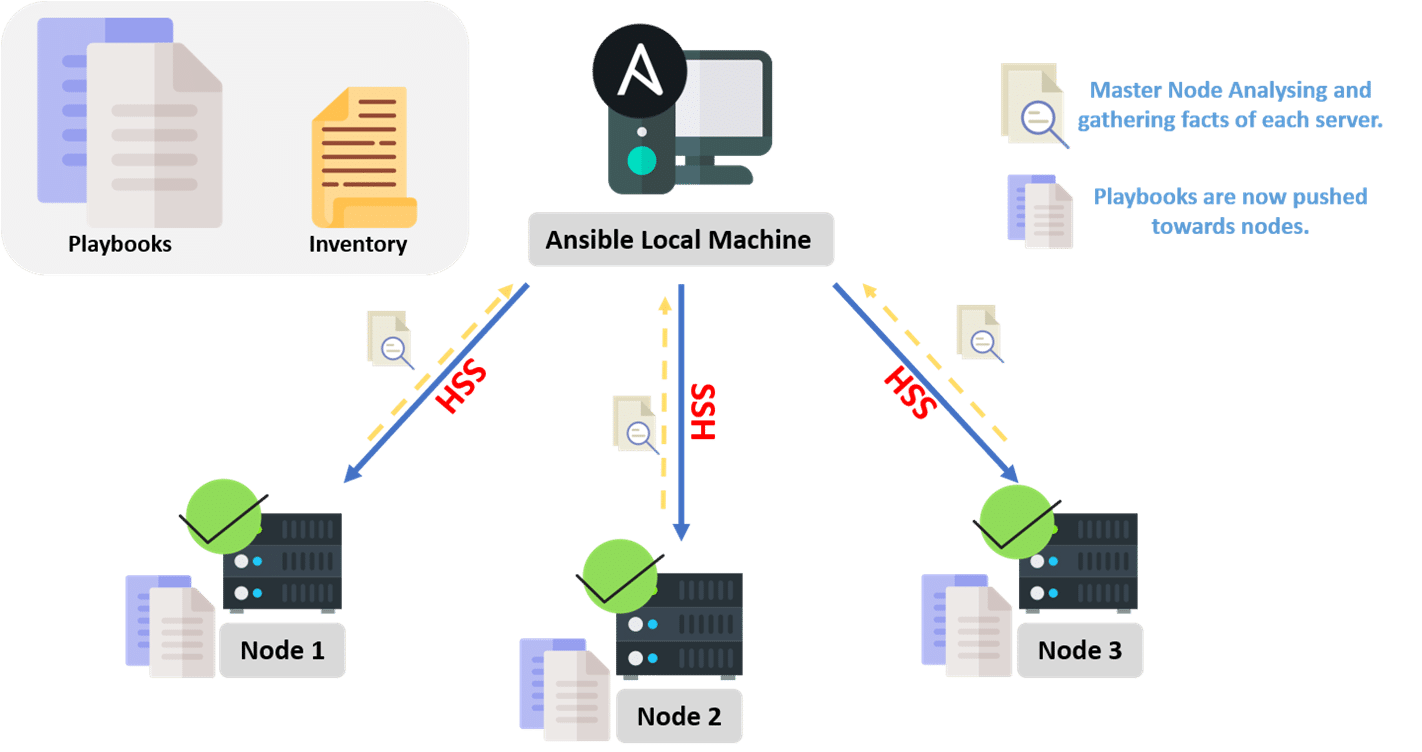
\includegraphics[scale=0.25]{pictures/ansible_node.png}\\
        \imagesource{https://intellipaat.com}
    \end{tabular}
    \caption{Koneksi Ansible menuju Node menggunakan SSH}
\end{figure}
\FloatBarrier

\section{Pendahuluan}
\subsection{Latar Belakang}
Klustering seiring berjalannya waktu semakin banyak digunakan di kalangan perusahaan tekno-logi. hal tersebut terjadi karena kemudahan yang diberikan oleh teknologi ini, untuk melakukan skalasi layanan dengan terhadap peluncuran perangkat lunak kepada konsumen setiap kali kebutuhan bertambah. Dimana dengan berkembangnya zaman digital, kebutuhan manusia untuk mendapatkan semakin banyak kekuatan komputasi semakin tidak dapat dielakkan. Tetapi terdapat batasan skalasi secara vertikal (menambah RAM, menambah CPU, menambah penyimpanan persisten di dalam satu sistem).

\vspace{0.2cm}
\noindent Dengan harga komoditas yang dibutuhkan sebagai bahan dasar pembuatan produk elektronik, inflasi, dan peningkatan biaya produksi barang elektronik, maka skalasi secara vertikal akan menjadi semakin sulit seiring dengan peningkatan harga komponen yang disebabkan oleh kualitas yang dibutuhkan \cite{electronic_cost}. Hal ini menyebabkan bertambahnya penggunaan perangkat komputasi murah yang dapat dengan mudah di produksi masal. dan diprediksi akan semakin meningkat seiring dengan berjalannya waktu \cite{raspi_market}.

\vspace{0.2cm}
\noindent Dengan meningkatnya penggunaan klustering, diperlukan pula sebuah sistem yang mampu memberikan solusi untuk pengelolaan node pada sebuah kluster yang dapat di otomatisasi. sehingga dapat dilakukan peluncuran aplikasi kepada konsumen secara efektif. Dan sistem tersebut harus mampu mengatasi \textit{error} ketika melakukan tugas yang telah diberikan sebelumnya, sehingga kemungkinan kerusakan terhadap seluruh jajaran sistem dapat dihindari.


\subsection{Rumusan Masalah}

\subsection{Tujuan}

\subsection{Manfaat}

\subsection{Batasan Masalah}
\section{Tinjauan Pustaka}

Kluster Merupakan sebuah teknologi yang dibuat sebagai upaya untuk mendapatkan kemampuan komputasi besar dengan harga murah. hal ini dilakukan dengan cara menghubungkan komputer, baik \textit{standalone}, terdistribusi, maupun paralel, dengan tujuan untuk membagi pekerjaan yang sebelumnya hanya dapat dilakukan oleh satu komputer saja secara bersamaan \cite{cloud_computing}. Untuk membagi tugas didalam setiap node, digunakan teknologi yang bernama Kontainerisasi.

\vspace{0.2cm}
\noindent Kontainerisasi memberikan kemampuan kepada pengembang untuk menciptakan aplikasi port-able \cite{containers}. menggunakan kontainerisasi, sebuah node dapat menjalankan berbagai macam tugas secara bersamaan, tanpa perlu mengkhawatirkan terjadinya konflik antar proses mengenai sumber daya yang ada. Seperti versi program yang berbeda, pustaka program yang tidak dapat ada secara bersamaan, dan kebutuhan akan integrasi kuat antar program di dalam kontainer. Selain itu, terdapat pula faktor keamanan dimana ketika sebuah kontainer terkontaminasi atau terkena serangan eksternal, tidak akan terjadi kerusakan pada kontainer lain karena isolasi yang diberikan oleh teknologi ini.

\vspace{0.2cm}
\noindent Penggunaan Raspberry Pi dalam server sederhana dan perangkat keras komputer juga meningkat seiring dengan berjalannya waktu. hal ini disebabkan oleh semakin tingginya angka pengembang aplikasi yang membutuhkan perangkat IoT dan lingkungan pengembangan murah untuk didapatkan dan/atau untuk digunakan sebagai sarana pembelajaran \cite{raspi_market}.

\subsection{Kubernetes}

Kubernetes memberikan sebuah platform open source portabel yang dapat diperluas untuk mengelola beban kerja dan layanan dalam container dalam bentuk orkestrasi, yang memfasilitasi konfigurasi deklaratif dan otomatisasi \cite{kubernetes_overview}. Didalamnya, terdapat Kluster, yang terdiri dari sekumpulan mesin pekerja, yang disebut node, yang menjalankan aplikasi dalam container. Setiap cluster memiliki setidaknya satu node pekerja \cite{kubernetes_components}. Node sendiri adalah sebuah perangkat keras maupun virtual yang bertugas menjalankan program didalam kontainer yang disebut Pods yang diluncurkan kedalam kluster yang diatur oleh sebuah \textit{controlplane} \cite{kubernetes_nodes}. Komponen komponen tersebut bersinergi dan bekerja sama dalam membentuk lingkungan perangkat lunak yang dapat terskala dan tumbuh secara horizontal. Sehingga dapat memberikan peluang baru bagi pengembang aplikasi dan administrator untuk merubah daya komputasi sesuai kebutuhan aplikasi pada saat tertentu dengan mudah dan mempermudah implementasi \textit{redundancy}.\\
\begin{figure}[htb!]
    \centering
    \begin{tabular}{ @{} r @{} }
        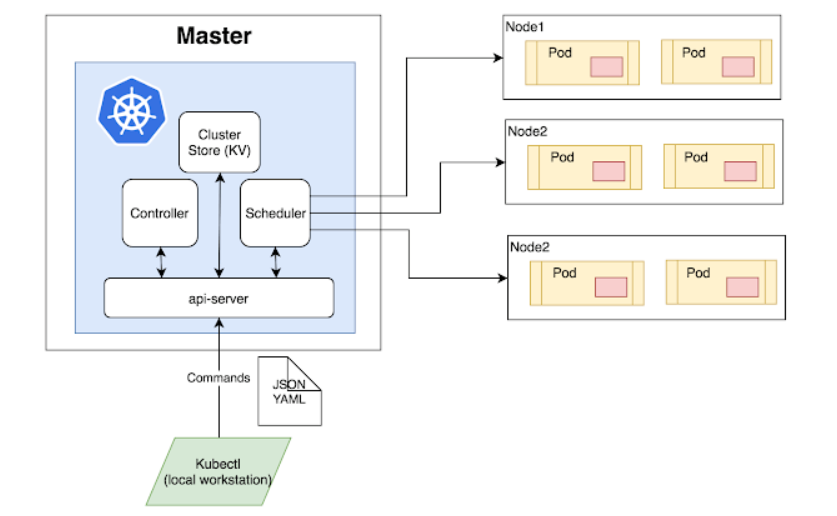
\includegraphics[scale=0.7]{pictures/k8s_diagram.png}\\
        \imagesource{https://www.eternalsoftsolutions.com}
    \end{tabular}
    \caption{Struktur Kubernetes (K8s)}
\end{figure}
\FloatBarrier

\subsection{Raspberry Pi}

Raspberry Pi adalah komputer kecil menggunakan arsitektur ARM murah yang berfungsi seperti komputer pada umumnya \cite{raspi}. Perangkat keras ini memberikan akses komputasi murah untuk menciptakan perangkat-perangkat lain seperti Internet of Things (IoT), Personal Computer (PC), dan Server. Dan karena mudahnya mendapatkan perangkat dalam jumlah yang besar, maka Raspberry Pi juga dapat digunakan sebagai node untuk dihubungkan menggunakan Kubernetes dengan K3s.
\begin{figure}[htb!]
    \centering
    \begin{tabular}{ @{} r @{} }
        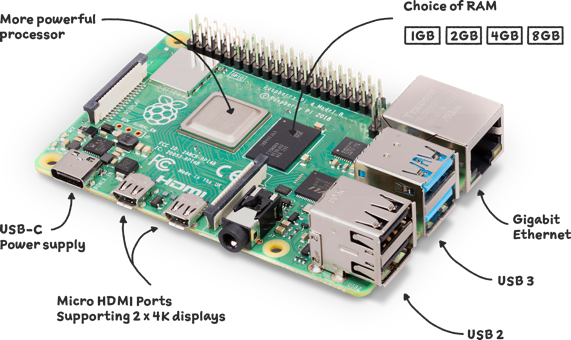
\includegraphics[scale=0.4]{pictures/raspi.png}\\
        \imagesource{https://www.raspberrypi.com/}
    \end{tabular}
    \caption{Komponen Raspberry Pi 4B}
\end{figure}
\FloatBarrier

\subsection{K3s}

K3s merupakan salah satu distribusi Kubernetes tersertifikasi dengan ketersediaan tinggi yang dirancang untuk beban kerja produksi di lokasi terpencil yang tidak diawasi, terbatas sumber daya, atau di dalam peralatan IoT \cite{k3s}. Portabilitas, ketersediaan, dan keringanan yang dimiliki oleh K3s didapatkan dengan memanfaatkan enkapsulasi seluruh komponen nya dalam satu proses. Yang hanya membutuhkan setidaknya 1vCPU dan 512MB RAM \cite{k3s_mk8s}. minimnya penggunaan sumber daya juga menjadi alasan utama pemilihan K3s jika dibandingkan dengan teknologi serupa seperti mK8s (MicroK8s) \cite{k3s_mk8s}. Dan karena enkapsulasi itu pula, tidak dibutuhkan pemasangan \textit{Docker Engine} secara terpisah didalam sistem yang menjalankan K3s.\\
\begin{figure}[htb!]
    \centering
    \begin{tabular}{ @{} r @{} }
        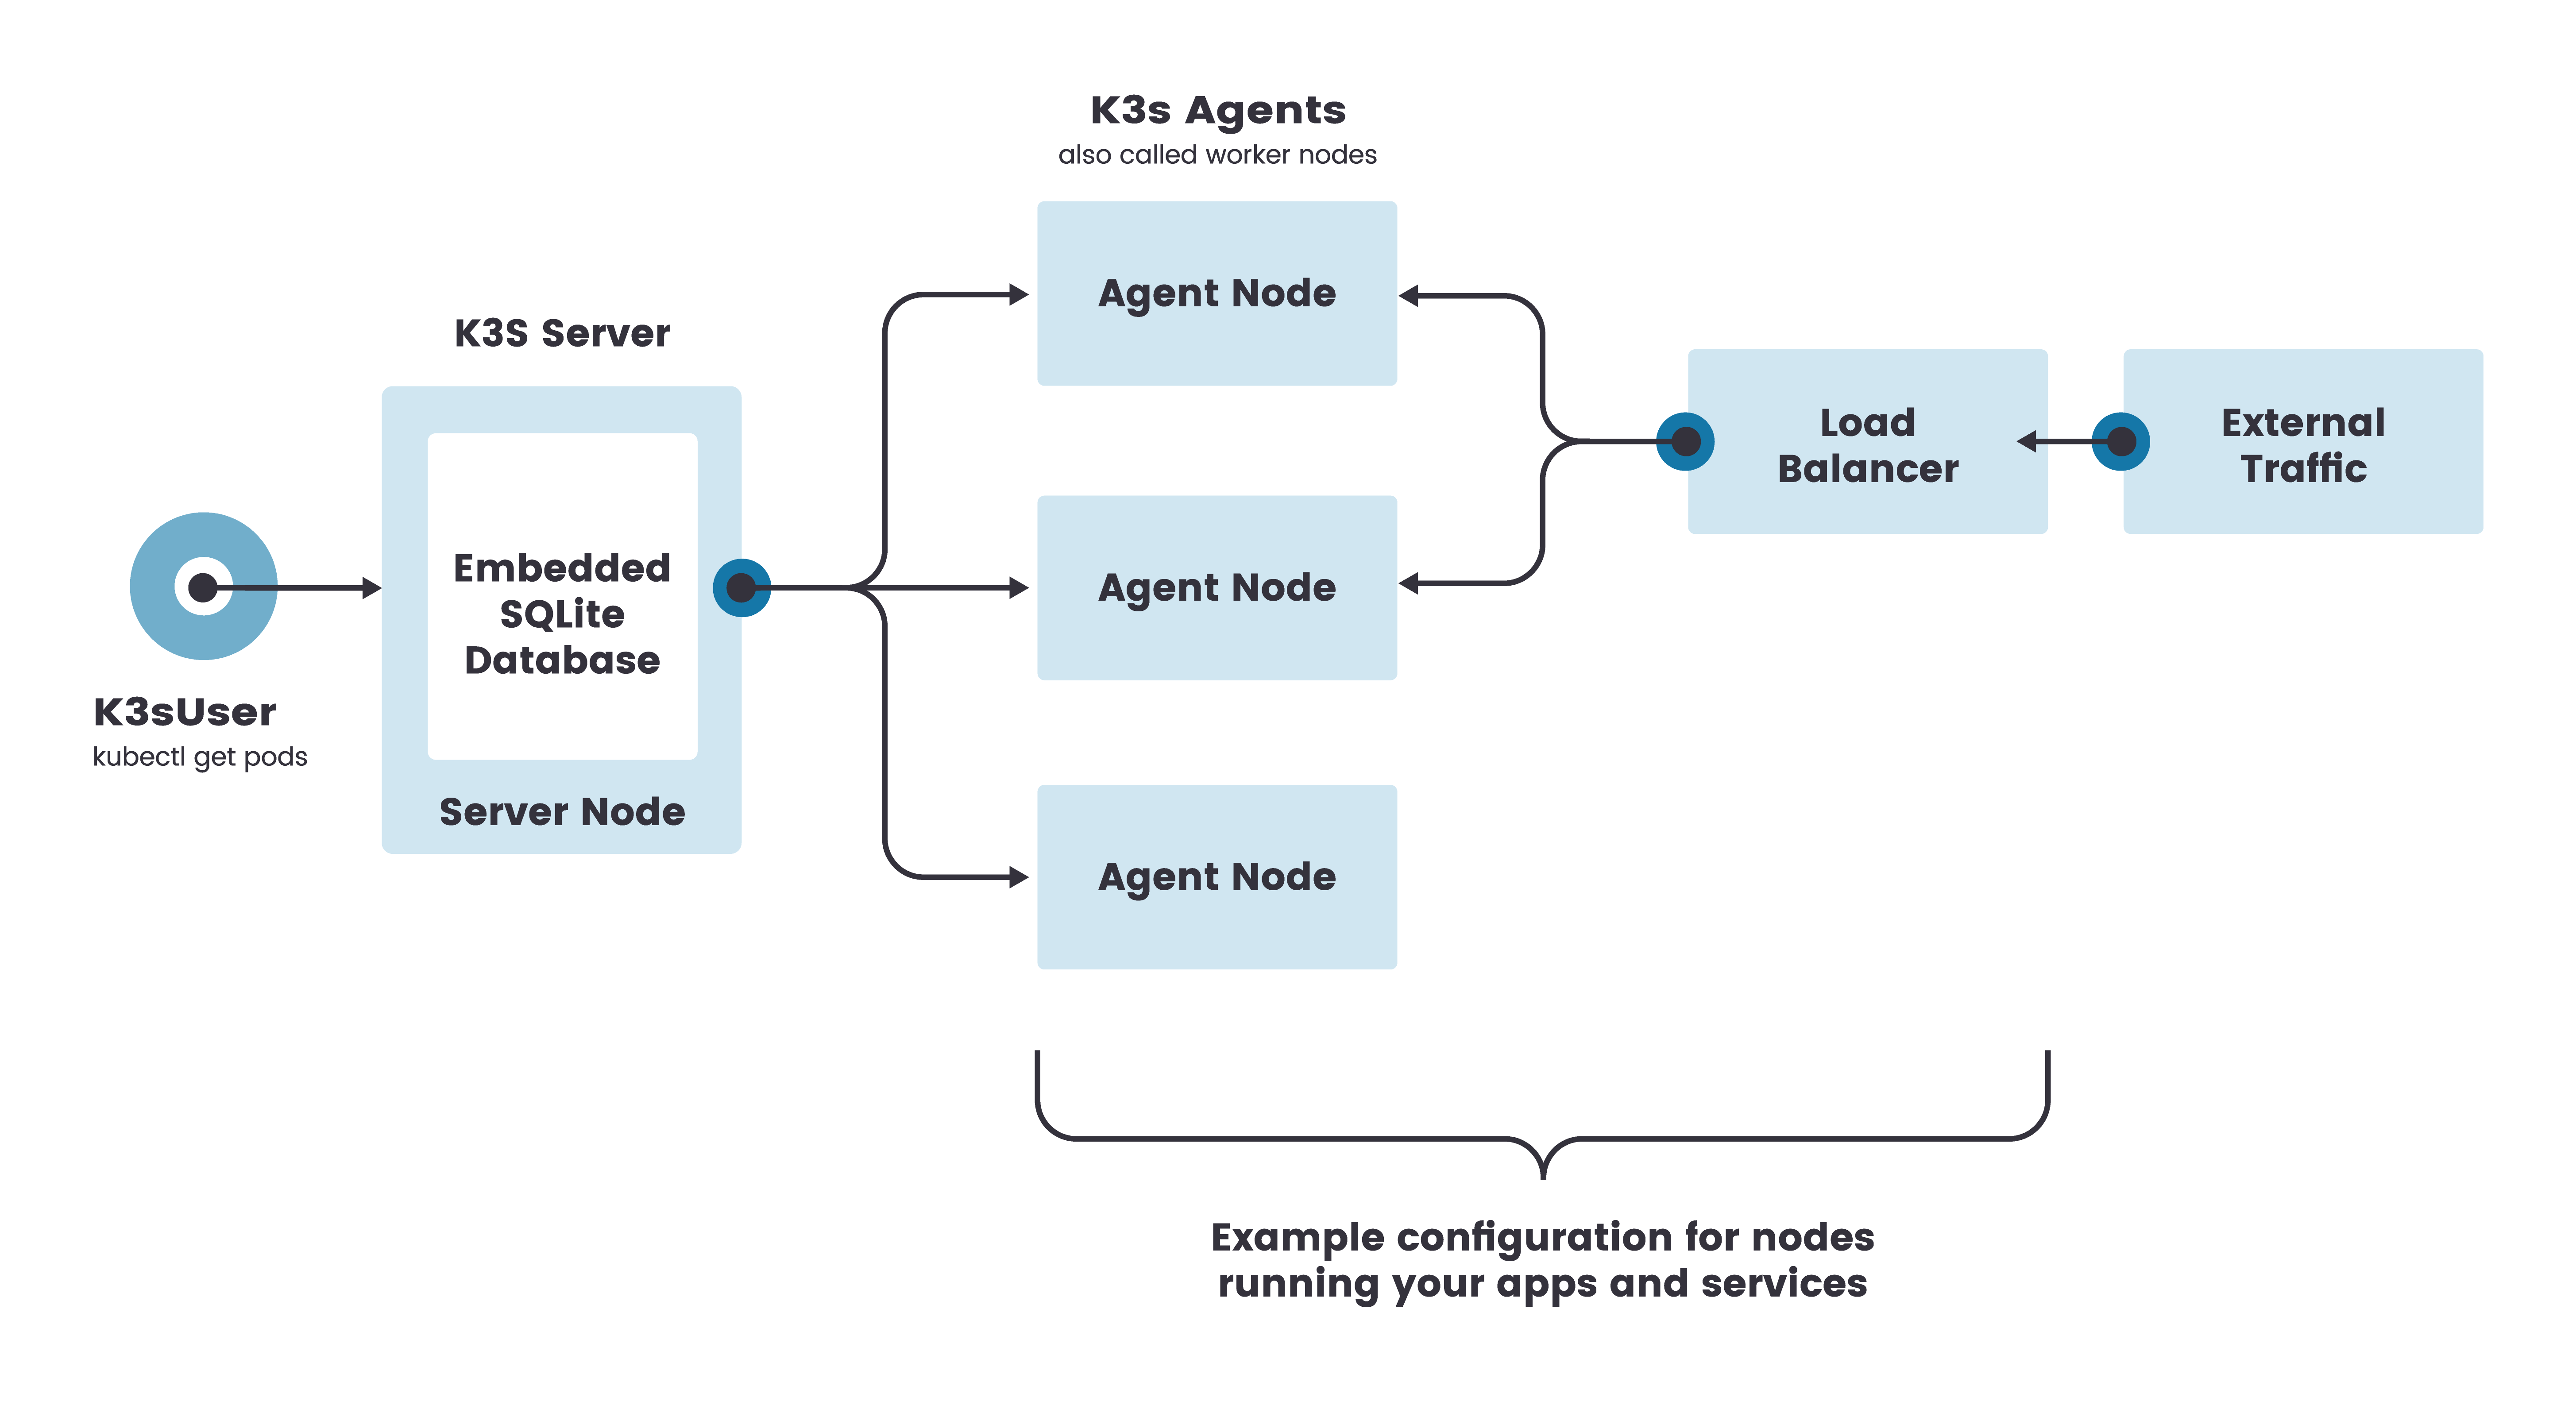
\includegraphics[scale=0.28]{pictures/k3s_diagram.png}\\
        \imagesource{https://nimblehq.co}
    \end{tabular}
    \caption{Struktur K3s}
\end{figure}
\FloatBarrier

\subsection{Ansible}

Ansible memiliki kemampuan untuk menghubungkan dan mempermudah proses pengaturan dan perawatan sistem pada saat peluncuran aplikasi. Karena Ansible mampu melakukan konfigurasi sistem, peluncuran perangkat lunak, dan mampu melakukan orkes-trasi kegiatan teknologi seperti \textit{Circular Integration/Circular Deployment} (CI/CD) \cite{ansible_docs}. menggunakan Ansible, pengaturan berulang yang harus dilakukan untuk setiap Node Rapsberry-Pi dapat di otomatisasi sehingga dapat mengurangi \textit{human error} dan meningkatkan efektifitas waktu.\\
\begin{figure}[htb!]
    \centering
    \begin{tabular}{ @{} r @{} }
        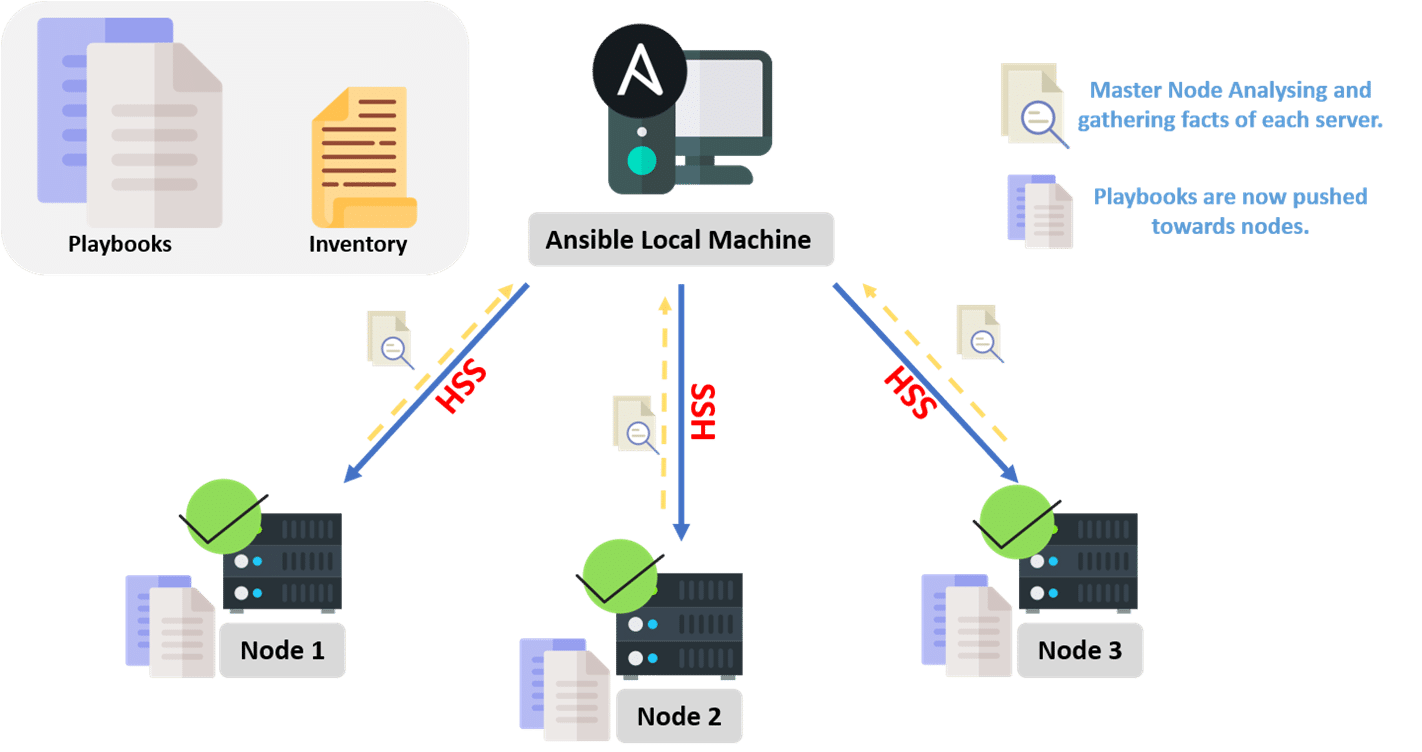
\includegraphics[scale=0.25]{pictures/ansible_node.png}\\
        \imagesource{https://intellipaat.com}
    \end{tabular}
    \caption{Koneksi Ansible menuju Node menggunakan SSH}
\end{figure}
\FloatBarrier

\section{Metode Penelitian}

\subsection{Studi Literatur}
Untuk menunjang pengerjaan penelitian ini, perlu dilakukan studi literatur untuk memberikan pengetahuan yang cukup untuk menyelesaikan penelitian ini. Studi literatur dilakukan dengan cara mengumpulkan dokumentasi dan pustaka yang berkaitan dengan penelitian ini. yaitu:
\begin{enumerate}
    \item Ansible
    \item K3s
    \item Raspberry Pi
\end{enumerate}

\subsection{Tipe Penelitian}
Tipe dari penelitian ini adalah penelitian eksploratif dan implementatif. Dimana akan dilakukan eksplorasi mengenai langkah-langkah yang dapat diambil untuk mengimplementasikan \textit{tech stack} hingga menjadi kluster yang dapat digunakan dalam lingkungan produksi.

\subsection{Rekayasa Kebutuhan}
Tabel berikut menjelaskan setiap kebutuhan yang dibutuhkan untuk melakukan penelitian.
\begin{table}[h]
    \begin{tblr}{
            hlines,
            vlines,
            row{1} = {bg=gray,fg=white,ht=1cm},
            columns = {halign=c},
            colspec = {Q[5cm]},
        }
        \textbf{Proses/ Kebutuhan} & \textbf{Perangkat Lunak/Keras}\\
        Node Master/Slave & Raspberry Pi \\
        Orchestrator & K3s \\
        Automation & Ansible \\
    \end{tblr}
    \centering
    \caption{Tabel kebutuhan penelitian}
\end{table}

\subsection{Rancangan Sistem}
Perancangan sistem dilakukan sebagai tahap awal untuk menggambarkan implementasi sisten secara sistematis dan terstruktur. Hal ini akan dilakukan ketika seluruh rekayasa kebutuhan untuk penelitian telah terpenuhi.
\begin{figure}[htb!]
    \centering
    \begin{tabular}{ @{} r @{} }
        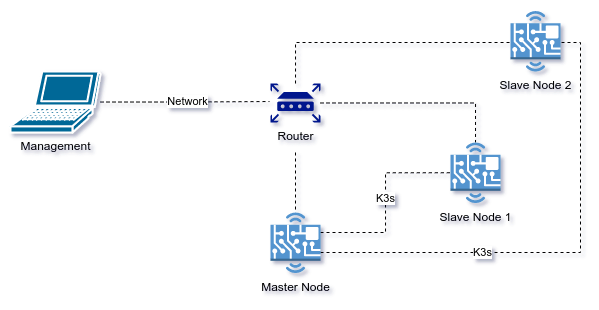
\includegraphics[scale=0.6]{pictures/rancangan_sistem.png}\\
    \end{tabular}
    \caption{Rancangan Sistem}
\end{figure}
\FloatBarrier
\noindent
Dari diagram perancangan diatas, terlihat beberapa node yang berupa Raspberry Pi terhubung pada sebuah router. Dimana router tersebut menghubungkan semua node kepada sebuah komputer manajemen untuk administrasi. Setiap node dapat berkomunikasi dengan node lain melalui Master Node menggunakan K3s dan komputer yang melakukan manajemen dapat mengakses secara langsung setiap node melalui jaringan yang disediakan melalui router.
\subsection{Skenario Pengujian dan Analisis Hasil}
Pengujian dilakukan dengan maksud untuk melihat kinerja sistem dan skalabilitas ketika ditambahkan node baru untuk digunakan oleh K3s dalam melakukan load balancing. Sehingga dapat dilihat efektifitas sistem ketika seluruh node telah menggunakan seluruh sumber dayanya dan memerlukan tenaga komputasi tambahan untuk dapat memproses lebih banyak permintaan.

\subsection{Pembentukan Kesimpulan}
Kesimpulan dibuat ketika informasi dari tahap tahap sebelumnya telah didapatkan dan dapat diringkas untuk membentuk ringkasan dari hasil penelitian.

\section{Research Plan}
State the long - and short -term objectives of your research program. Outline specific projects planned to meet these goals, including the timelines for completion of each stage, methods to be used, and dissemination of results. 

\section{Resources}
Provide details on the instrumentation and materials needed, along with the estimates of human resources required for each project/activity throughout the lifetime of the project
\cite{cloud_computing}

\newpage
\section*{Referensi}
\addcontentsline{toc}{section}{Referensi}
\printbibliography[heading=none]

\end{document}